\section{Results and Discussion}
\subsection{Zero Preload --- Young's Modulus of Bolt}
\label{sec:zero_preload_youngs_modulus}
The Young's Modulus for the bolt, $E_b$, was determined to be 205 $\pm 4.70$ GPa. The zero-preload trial was used to determine Young's Modulus for the bolt. The nut was tightened to finger tight, ensuring the preload force is negligible. The external load in this case is then equivalent to the total load on the bolt. The output voltage of the strain gauge was used to determine the strain in the bolt. Figure \ref{fig:external_load_vs_bolt_strain} shows the plot of the bolt strain against the external load and its linear regression through the origin. 
\begin{figure}[h]
    \centering
    \begin{minipage}{0.50\textwidth}
        \centering
        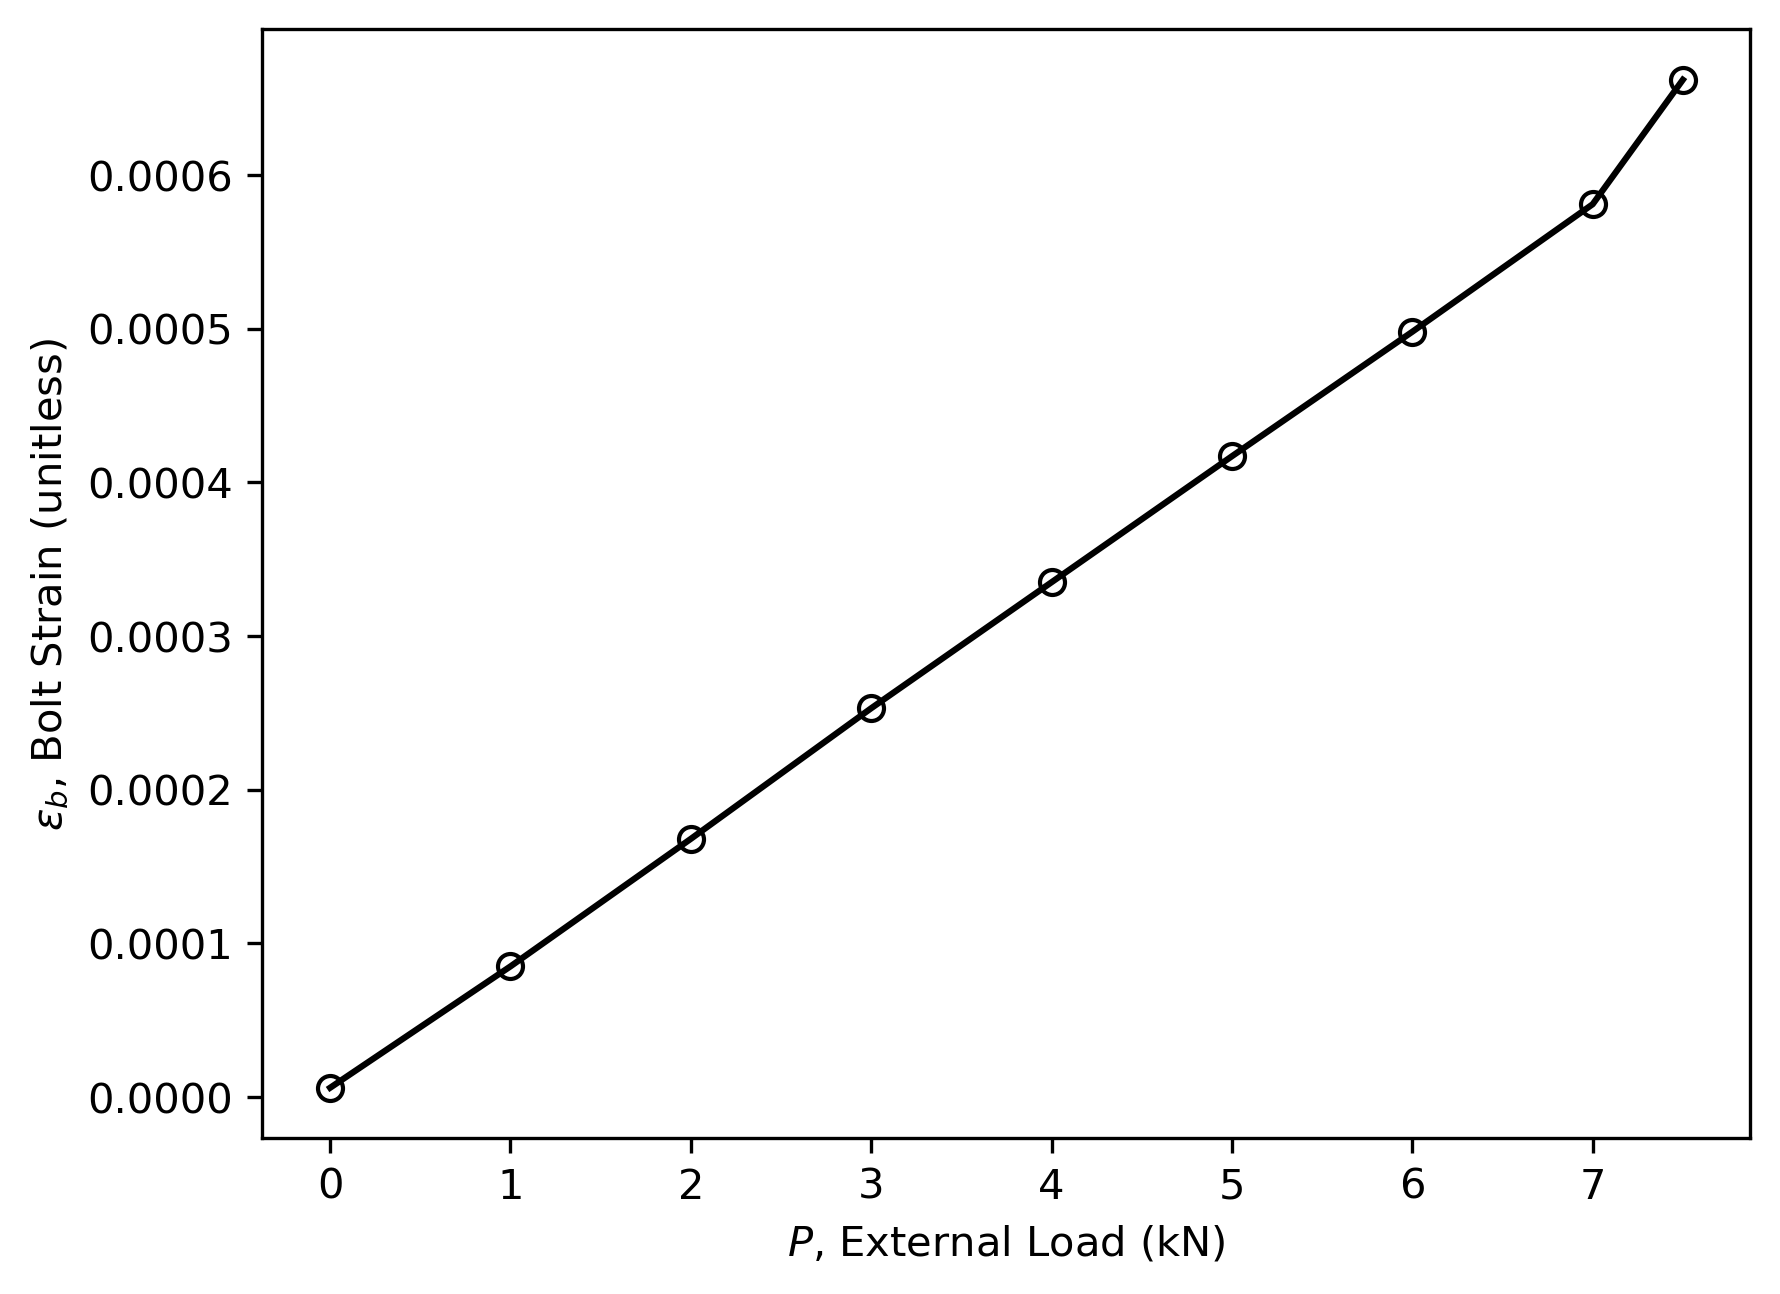
\includegraphics[width=0.9\textwidth]{Sections/Figures/external_load_vs_bolt_strain.png}
        \caption{External Load vs. Bolt Strain}
        \label{fig:external_load_vs_bolt_strain}
    \end{minipage}\hfill
    \begin{minipage}{0.50\textwidth}
        \centering
        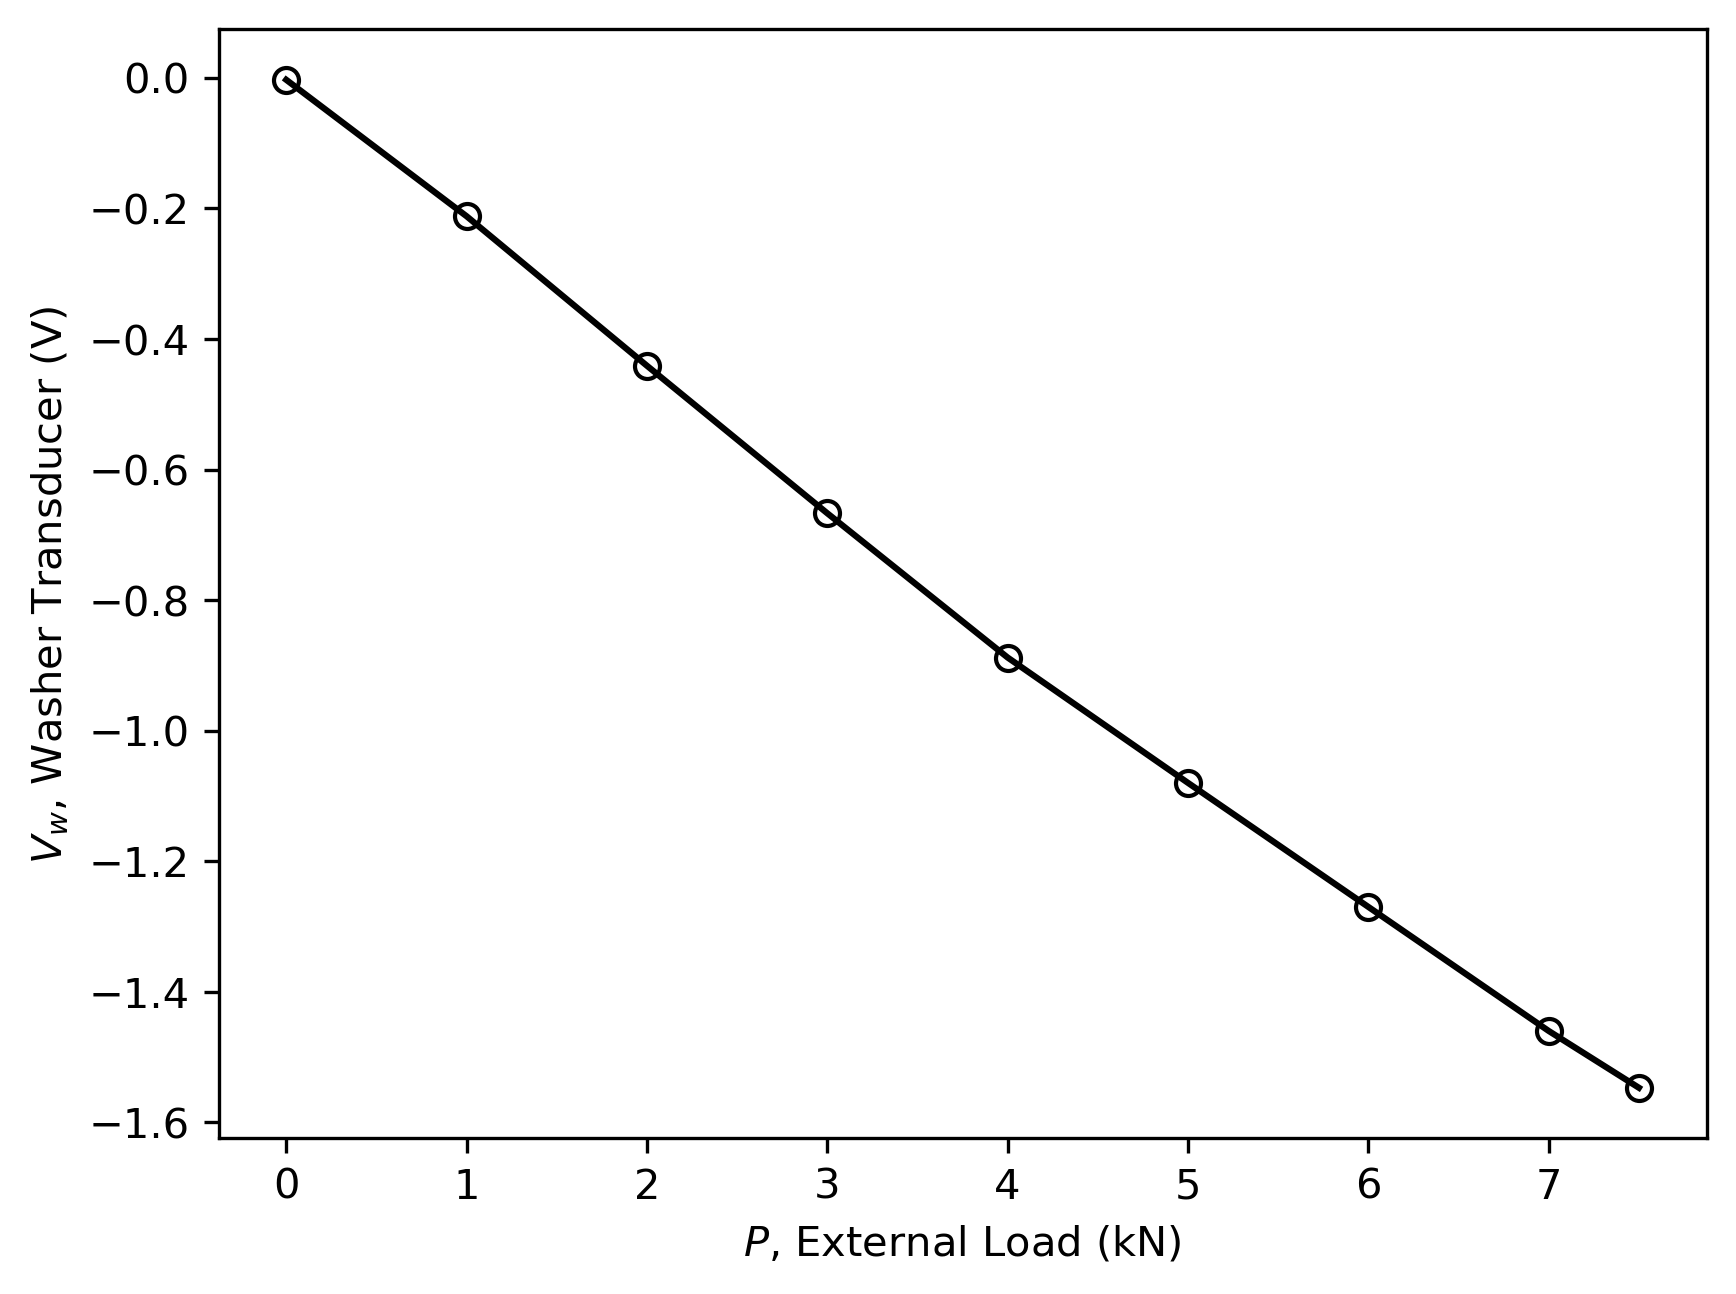
\includegraphics[width=0.9\textwidth]{Sections/Figures/external_load_vs_washer_transducer.png}
        \caption{External Load vs. Washer Transducer}
        \label{fig:external_load_vs_washer_transducer}
    \end{minipage}
\end{figure}

Using the slope from Figure \ref{fig:external_load_vs_bolt_strain} coupled with Eqs. (\ref{eq:stress_strain}) and (\ref{eq:force_area}), the Young's Modulus for the bolt, $E_b$, was determined to be 205 $\pm 4.70$ GPa. The linear regression had an $R^2 =  0.9992$, indicating a strong linear relationship between the external load and the bolt strain, agreeing with the stress-strain theory. The uncertainty was determined using a 95\% confidence interval. The error of the modulus was relatively small, adding confidence to the results. Sample calculations and error analysis can be found in Appendix \ref{app:zero_preload_analysis}.

\subsection{Zero Preload --- Washer Transducer Calibration}
The relationship between the washer output, $V_{o, w}$, and the external load (kN), $P$, was determined to be $V_{o, w} = -2.11 \times 10^{-4}P$. Again, the zero-preload trial was used to determine the washer calibration. The nut was tightened to finger tight, ensuring the preload force is negligible. The voltage output from the washer during the zero-preload trial was used to determine the washer calibration. Figure \ref{fig:external_load_vs_washer_transducer} shows the plot of the experimental data and its linear regression through the origin. The regression had an $R^2 = 0.9994$, indicating a strong linear relationship between the external load and the washer transducer.

Using the regression and Eq. (\ref{eq:strain_bridge}), the relationship between the washer strain, $V_{o, w}$, and the external load (kN), $P$, was determined to be $V_{o, w} = -2.11 \times 10^{-4}P$. The negative sign in the equation indicates that the washer compresses as the external load increases, consistent with expectations. The high $R^2$ value indicates a strong linear relationship between the washer strain and the external load, adding confidence to the results. Sample calculations can be found in Appendix \ref{app:zero_preload_analysis}.

\subsection{Zero Loading --- Torque and Preload}
\label{sec:zero_loading_torque_preload}
The relationship between torque and preload was $F_i = 0.636T$. The nut was tightened to various torques using a torque wrench, and the strain gauge output was used to determine the preload. The output voltage from the bolt transducer, coupled with Eq. (\ref{eq:strain_bridge}) and (\ref{eq:stress_strain}) was used to determine the preload on the bolt. Figure \ref{fig:torque_vs_preload} shows the plot of the experimental data and its linear regression. The regression had an $R^2 = 0.9995$, indicating a strong linear relationship between the torque and the preload. 

To calculate the preload, the modulus of elasticity, $E_b$, and strain transducer reading $V_b$ were used. The error for the preload by propagation of uncertainty. The uncertainty for the transducer reading was determined from a repeatability test. The major source of error was the strain transducer reading, which dominated the uncertainty. Sample calculations and error analysis can be found in Appendix \ref{app:preload_vs_torque_analysis}.

The results are expected as a linear relationship between torque and preload was discussed in Section \ref{sec:torque_for_preloading} by Eq. (\ref{eq:torque_constant}). The uncertainty of the 125 in-lb torque wrench had the highest uncertainty of $\pm 0.422$ kN, which was $4.60\%$ relative uncertainty. The absolute uncertainty was inversely proportional to the strain transducer reading. This means that the uncertainty of the first measurement was relatively large, and decreases as the strain transducer reading increases. The main source of error was the transducer reading. The relative error of $4.60\%$, along with the $R^2 = 0.9995$, adds confidence to the results. 
\begin{figure}[h]
    \centering
    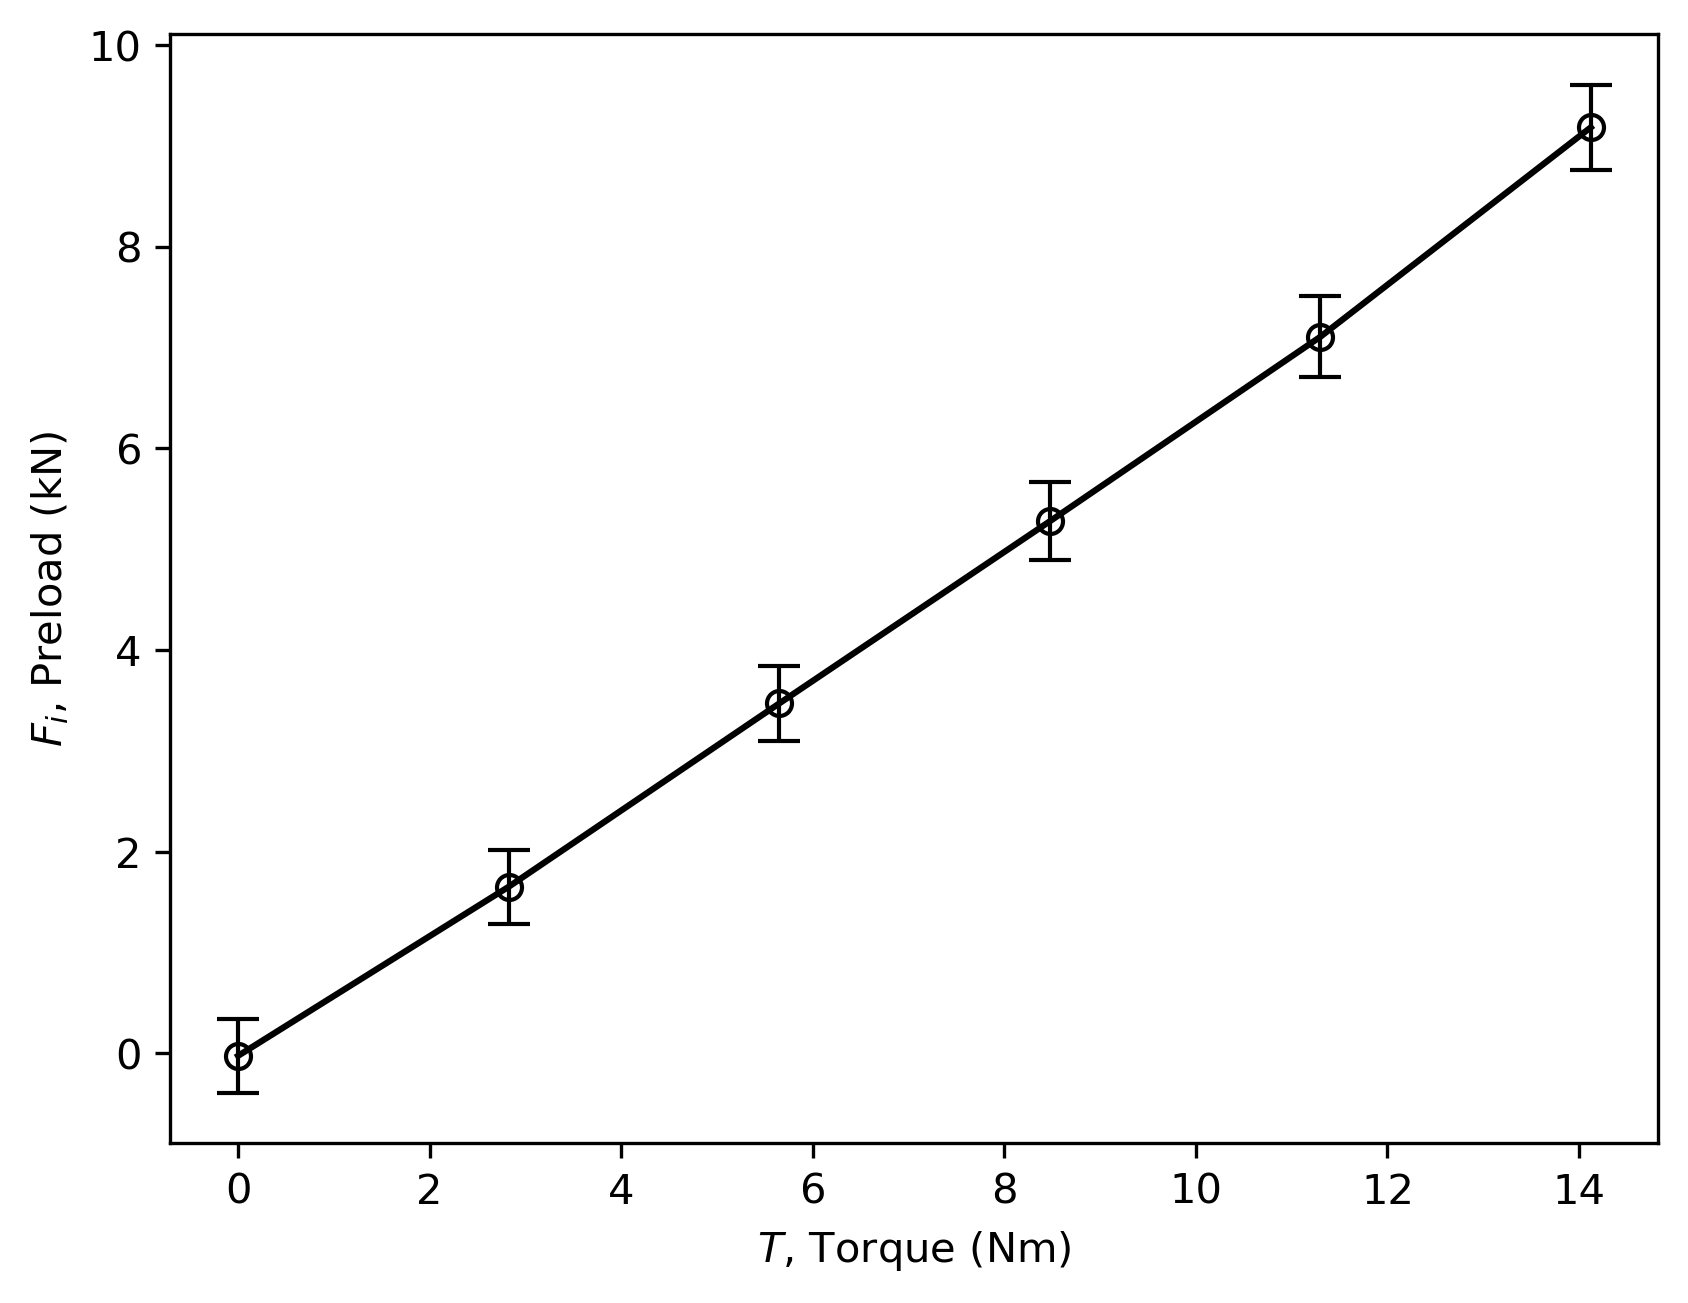
\includegraphics[width=0.5\textwidth]{Sections/Figures/torque_vs_preload.png}
    \caption{Torque vs. Preload}
    \label{fig:torque_vs_preload}
\end{figure}

\subsection{Zero Loading --- Torque Coefficient}
The torque coefficient, $K$, was determined to be $0.167$. This was obtained using the results from Section \ref{sec:zero_loading_torque_preload} combined with Eq. (\ref{eq:torque_constant}). This value was within the expected range of $0.1 - 0.2$, agreeing with theory. The confidence is high due to the $R^2 = 0.9995$ and the low relative uncertainty of $4.60\%$. This result will be used later to determine the preload in later sections. While uncertainty was not calculated, future work utilizing the standard error of the slope along with a confidence of 95\% could be used to determine the torque coefficient uncertainty. Sample calculations can be found in Appendix \ref{app:zero_preload_analysis}.

\subsection{No Gasket, Static Loading --- Torsional Loading}
Negligible evidence of torsional loading was found during the shakedown test. A shakedown test was performed by ramping the external load from 0 kN to 7.5 kN back down to 0 kN three times in succession. The voltage at the end of each ramp was recorded. The strain transducer reading varied by $\pm 0.005$ V, which was the same magnitude as the resolution of the strain transducer. This indicates that the bolt was not subjected to any torsional loading. The results were consistent with expectations, as the bolt was not subjected to any torsional loading. Sample calculations can be found in Appendix \ref{app:shakedown_test}.

\subsection{Bolt Stiffness}
\begin{figure}[h]
    \centering
    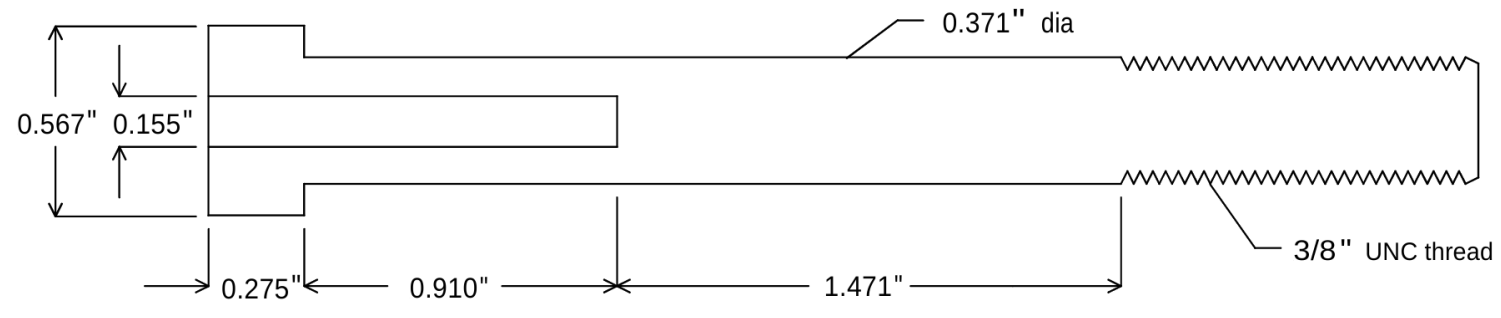
\includegraphics[width=0.5\textwidth]{Sections/Figures/bolt member drawing.png}
    \caption{Cross Section of the Strainsert Type W Bolt Transducer}
    \label{fig:bolt_member_drawing}
\end{figure}
The stiffness of the bolt was determined to be $k_b = 209$ MN/m. The bolt was divided into three sections, as shown in Figure \ref{fig:bolt_member_drawing}. The stiffness of each section was determined using Eq. (\ref{eq:member_stiffness}). The stiffness of sections 1, 2, and 3 were determined to be 510 MN/m, 383 MN/m, and 4834 MN/m, respectively. The total bolt stiffness was then determined using Eq. (\ref{eq:member_stiffness_series}). This value will be used later to determine the experimental and theoretical stiffness of the member. While uncertainty analysis was not conducted, the largest contributor to error was the uncertainty from modulus of elasticity, $E_b$. Sample calculations can be found in Appendix \ref{app:bolt_stiffness}.

\subsection{Theoretical Joined Member Stiffness}
The theoretical stiffness of the joined members was determined to be $k_m = 2222$ MN/m. The stiffness of the member was determined using Eq. (\ref{eq:member_stiffness_theory}). This assumes the angle of the stress distribution was 45$^\circ$. This will be used as the expected value for the member stiffness, and will be compared to the experimental value later. Sample calculations can be found in Appendix \ref{app:theoretical_member_stiffness}.

\subsection{Static Loading --- With and Without Gasket}
\label{sec:static_loading_with_without_gasket}
\begin{figure}[h]
    \centering
    \begin{minipage}{0.50\textwidth}
        \centering
        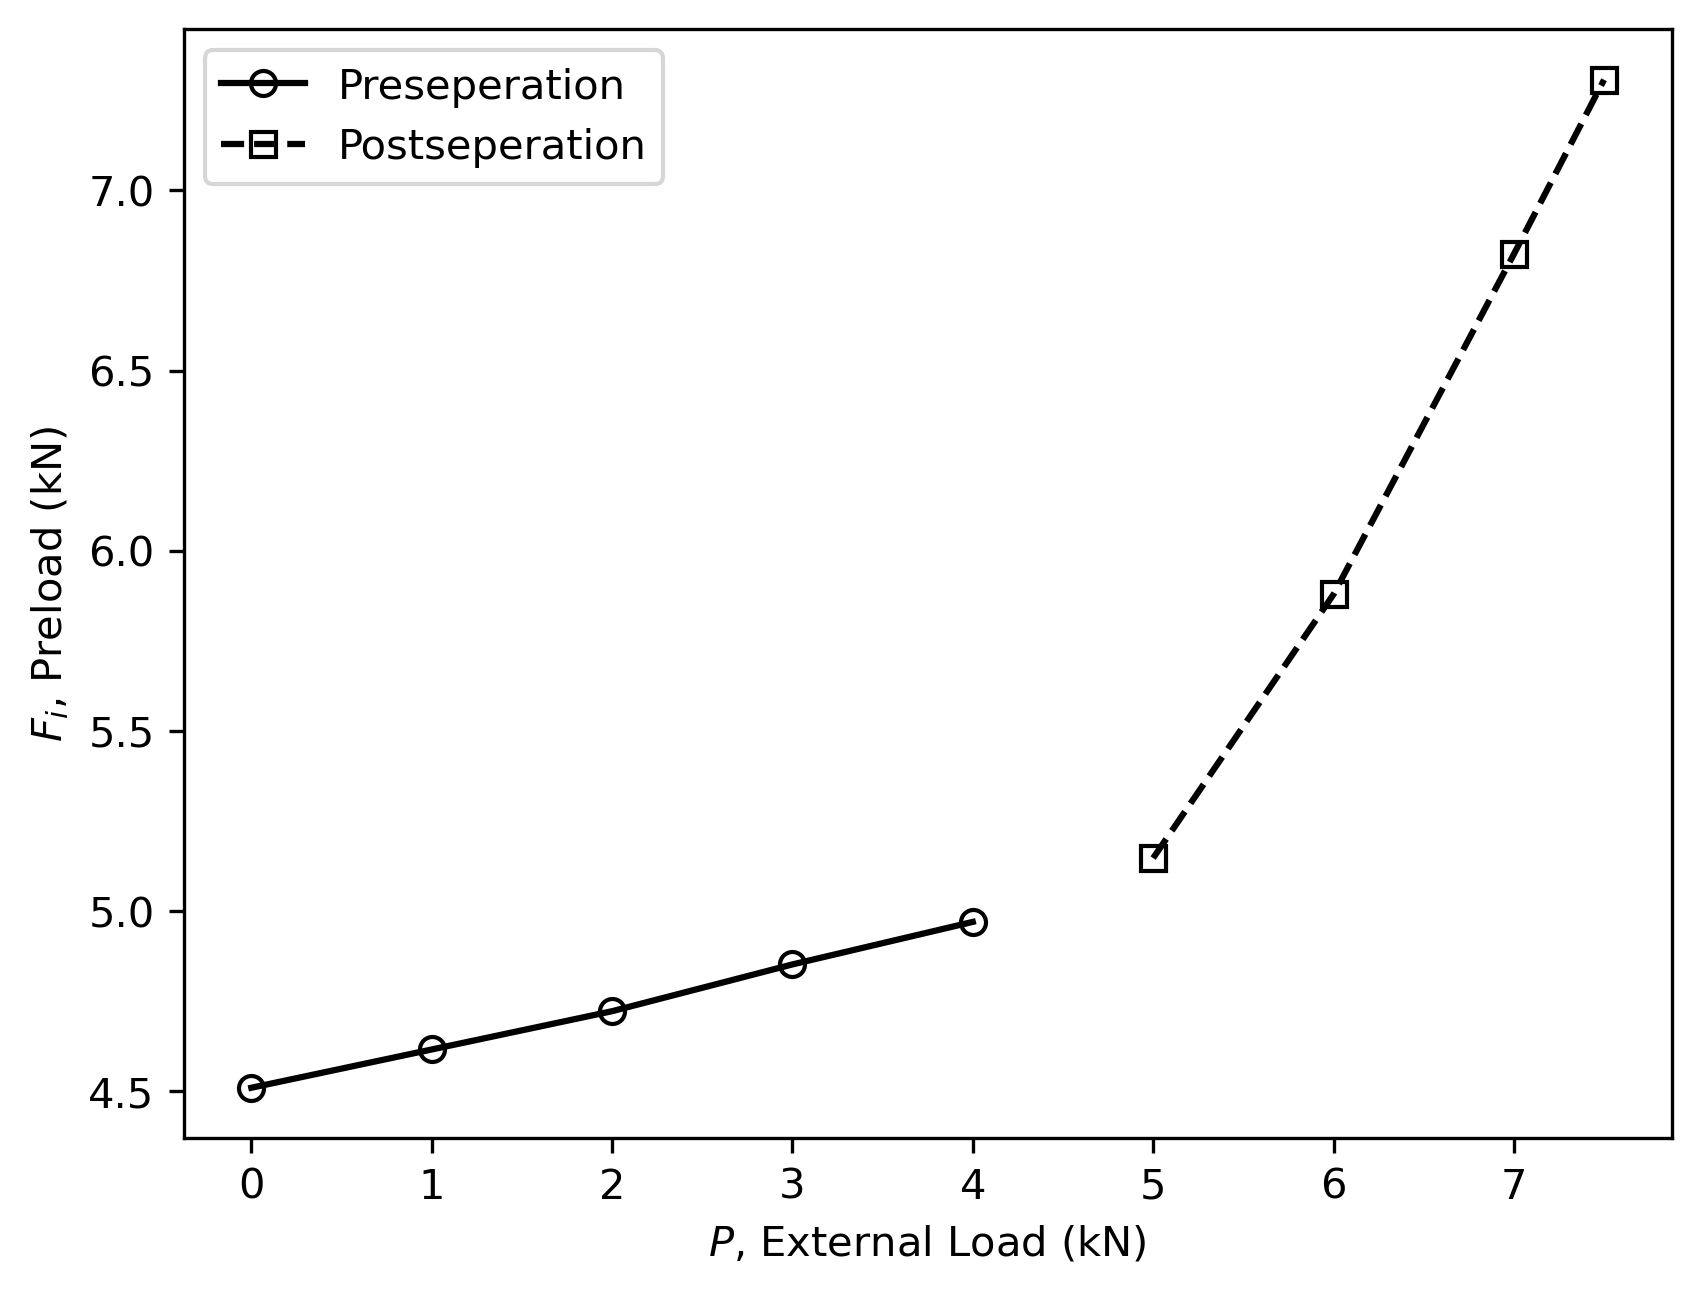
\includegraphics[width=0.9\textwidth]{Sections/Figures/without_gasket_preseperation_vs_postseperation.png}
        \caption{Static loading of bolted connection without gasket}
        \label{fig:without_gasket_loading}
    \end{minipage}\hfill
    \begin{minipage}{0.50\textwidth}
        \centering
        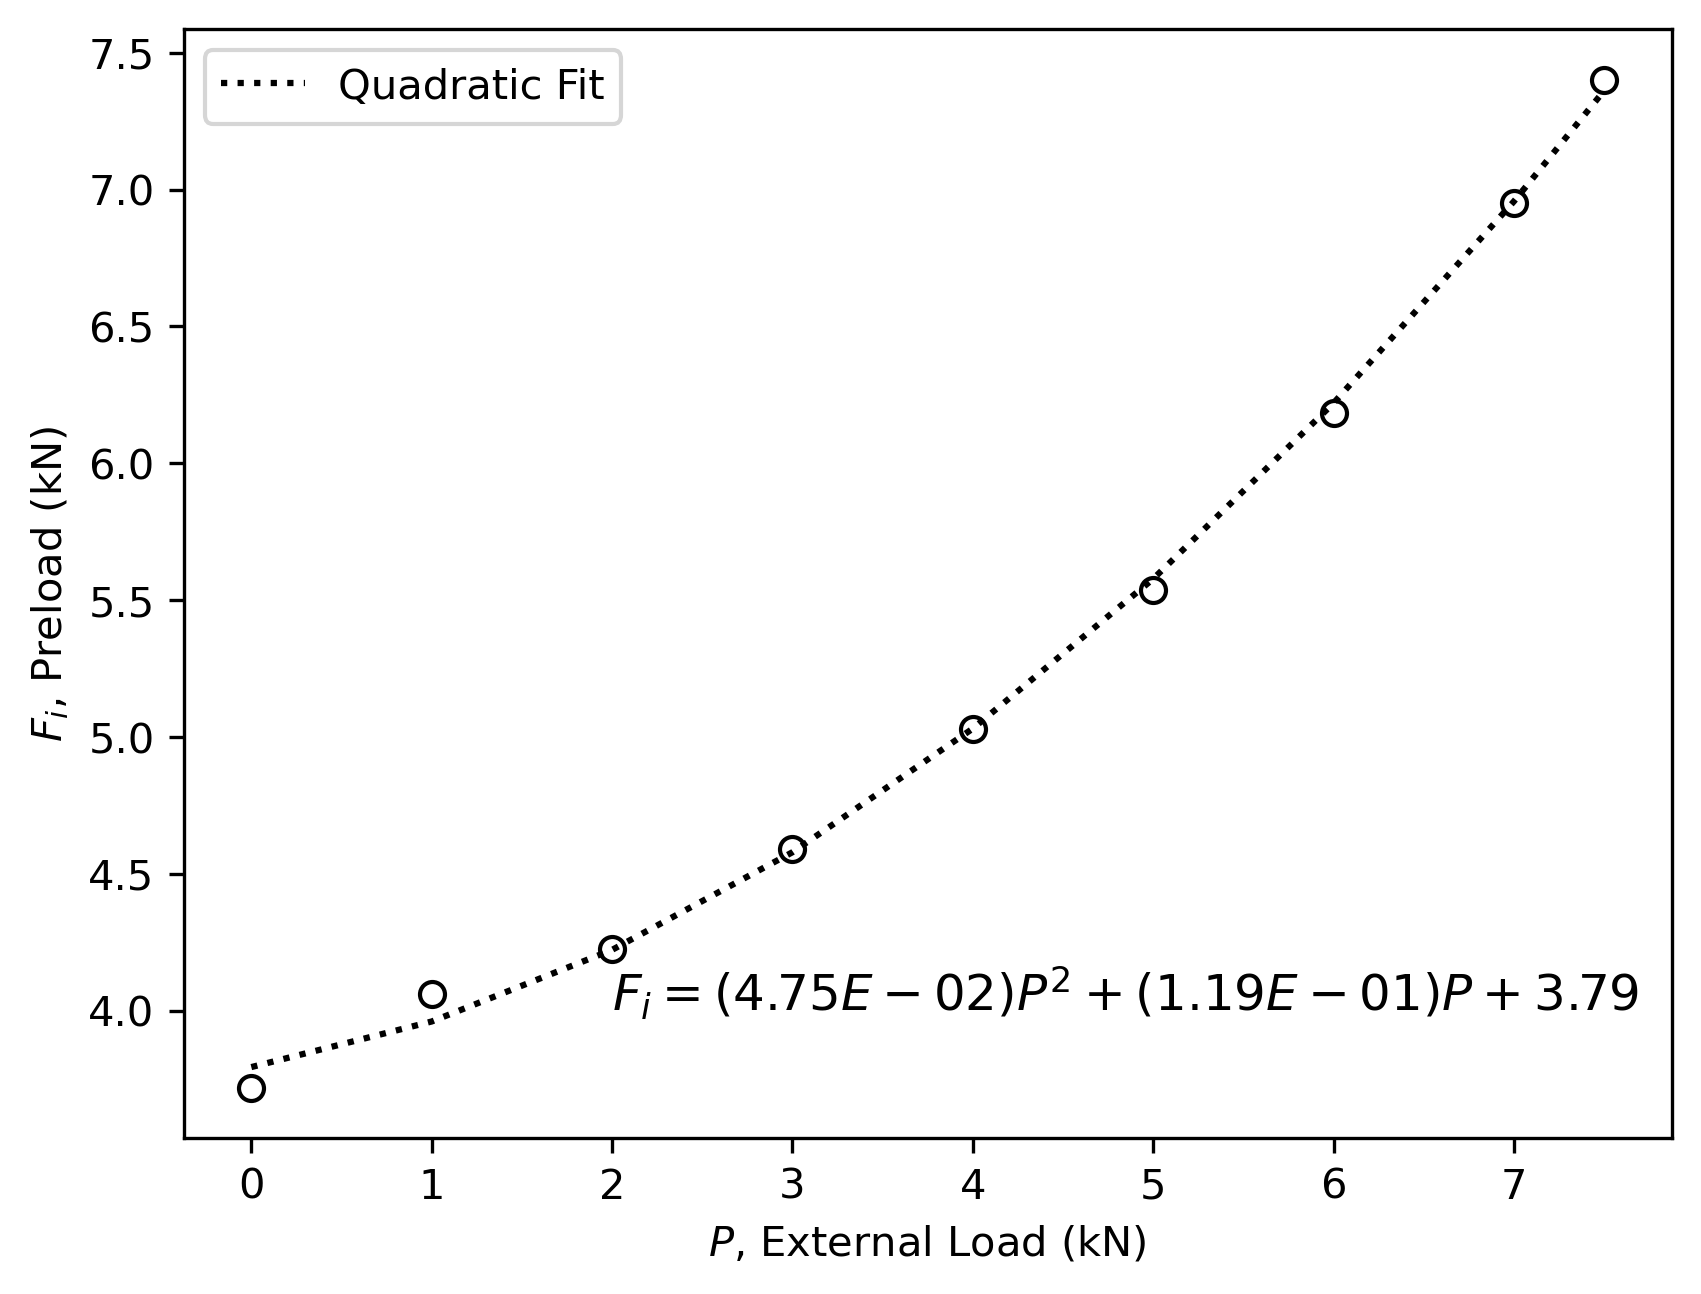
\includegraphics[width=0.9\textwidth]{Sections/Figures/with_gasket_preseperation.png}
        \caption{Static loading of bolted connection with gasket}
        \label{fig:with_gasket_loading}
    \end{minipage}
\end{figure}
% \noindent Two sets of trials were conducted at a torque setting of 60 in-lb: one with a gasket and one without. Various external loads between 0 kN and 7.5 kN were applied to the bolted connection. The voltage output from the bolt transducer was used to determine the bolt strain. The bolt strain was then used to determine the bolt preload using Eq. (\ref{eq:stress_strain}). The results are shown in Figures \ref{fig:without_gasket_loading} and \ref{fig:with_gasket_loading}. The differerence between the gasket and no gasket trials was the presence of a seperation point. 

The no gasket trial shown in Figure \ref{fig:without_gasket_loading} had a linear relationship between the external load and the bolt strain. Two regressions of $F_{b, \text{pre}} = 0.1157 P + 4.5022$ and $F_{b, \text{post}} = 0.8687 P + 0.7507$ were used to fit the data. Two regressions were required due to the separation point at 4.98 kN. The pre and post seperation $R^2$ values were 0.9983 and 0.9958, respectively, indicating a strong linear relationship between the external load and the bolt strain. An increase in the bolt force for an external load was observed in the separation point trial. This is expected as the bolted connection was no longer in contact with the members. The quadratic fit was good, with an $R^2 = 0.9985$, indicating a strong quadratic relationship between the external load and the bolt strain.

The gasket trial shown in Figure \ref{fig:with_gasket_loading} had a quadratic relationship between the external load and the bolt strain. The regression was found to be $F_{b, \text{gasket}} = 0.0475 P^2 + 0.119 P + 3.794$. The quadratic fit was good, with an $R^2 = 0.9985$, indicating a strong quadratic relationship between the external load and the bolt strain. In general, the gasket trial had a lower bolt force for a given external load, indicating the gasket was effective in reducing the bolt force. The separation point was not observed in the gasket trial, as the effect of the gasket prevented the members from separating within the tested loads. Future work in testing values beyond 7.5 kN could be used to determine the separation point of the gasket trial.

The results were consistent with expectations. The no gasket had a steeper slope than the gasket trial, indicating a higher stiffness. The separation point was observed in the no gasket trial, but not in the gasket trial. The $R^2$ values were high, indicating a strong linear and quadratic relationship between the external load and the bolt strain.

The effect of the gasket reduces bolt force for a given external load. The gasket also helps to prevent the members from separating. The separation point was observed in the no gasket trial, but not in the gasket trial. The $R^2$ values were high, indicating a strong linear and quadratic relationship between the external load and the bolt strain. 

\subsection{Experimental Joined Member Stiffness Without Gasket}
The stiffness of the joined members was experimentally determined to be $k_m = 1600$ MN/m. The stiffness of the member was determined using the preseparation  regression from Section \ref{sec:static_loading_with_without_gasket}. The constant $C$ was determined to be $0.1157$ from the preseparation regression. This value was then used to determine the experimental stiffness of the member using Eq. (\ref{eq:constant_C}). 

The relative error between the theoretical value of $k_m = 2222$ MN/m and the experimental value of $k_m = 1600$ MN/m was $28.0\%$. The error was relatively large, indicating a large discrepancy between the theoretical and experimental values. While a portion of the error was due to uncertainty from the modulus of elasticity, $E_m$, and strain transducer uncertainty, $V_b$, this does not account for the large discrepancy. A key assumption made in the theoretical calculation was that the stress distribution was 45$^\circ$. This was never verified, and could be a source of error. Future work could be done to verify the stress distribution angle. Sample calculations can be found in Appendix \ref{app:experimental_member_stiffness}.

\subsection{Experimental Joined Member Stiffness With Gasket}
Determining the joined member stiffness with gasket is difficult. The lack of a separation point makes it difficult to calculate the stiffness of the member. In addition, the theory was developed for a linear relationship between bolt force and external load. Since the gasket is made of a softer material, it could be expected that the stiffness would decrease. This is beneficial as the gasket would help to reduce the bolt force for a given external load. Future work in developing a model that accounts for quadratic fits as well as increasing the range of loads tested could be used to determine the stiffness of the member with gasket.

\subsection{Static Loading --- Separation Point}
The external load at the separation point for the experimental and theoretical values were determined to be 4.98 kN and 4.67 kN, respectively. The experimental separation point was determined by equating the preseparation and postseparation regressions from Section \ref{sec:static_loading_with_without_gasket}. The theoretical separation point was determined using Eq. (\ref{eq:joint_separation}) using the experimental $k_b$ and theoretical $k_m$. The relative error between the experimental and theoretical separation points was $6.78\%$. This error was modestly small. The main discrepancy came from the difference in the experimental and theoretical stiffness of the member, with a relative error of $28.0\%$. Despite the large difference in the stiffness of the member, the separation point was relatively close. Future work in determining the stress distribution angle could be used to determine the separation point with higher accuracy and confidence. Sample calculations can be found in Appendix \ref{app:joint_seperation}.
\begin{table}[h]
    \centering
    \caption{Dynamic Loading Summary for Various Torques and Gasket Conditions}
    \label{tab:dynamic_loading_main_results}
    \begin{tabular}{p{0.10\textwidth}C{0.10\textwidth}C{0.15\textwidth}C{0.15\textwidth}C{0.15\textwidth}C{0.15\textwidth}}
    \toprule
    & Torque, $T$ & Max Stress, $\sigma_{\text{max}}$ & Min Stress, $\sigma_{\text{min}}$ & Mean Stress, $\sigma_{\text{mean}}$ & Alternating Stress, $\sigma_{\text{a}}$ \\
    & (in-lb) & (MPa) & (MPa) & (MPa) & (MPa) \\
    \midrule
    \multirow{4}{*}{With Gasket} & 0 & 105.035 & 61.804 & 83.420 & 21.615 \\
    & 60 & 110.300 & 88.864 & 99.582 & 10.718 \\
    & 75 & 124.101 & 110.488 & 117.295 & 6.806 \\
    & 125 & 174.584 & 167.250 & 170.917 & 3.667 \\
    \midrule
    \multirow{4}{*}{No Gasket} & 0 & 105.330 & 62.098 & 83.714 & 21.616 \\
    & 60 & 106.347 & 84.153 & 95.250 & 11.097 \\
    & 75 & 108.671 & 101.337 & 105.004 & 3.667 \\
    & 125 & 166.652 & 163.258 & 164.955 & 1.697 \\
    \bottomrule
    \end{tabular}
\end{table}
\subsection{Dynamic Loading --- Mean and Alternating Stresses}
\indent The results are summarized in Table \ref{tab:dynamic_loading_main_results}. The mean stress increases as torque increases and the alternating stress decreases as torque increases. The gasket generally increased the mean stress and alternating stress. In this test, the MTS testing machine was utilized to apply an alternating load of 1.25 kN at 0.3 Hz frequency. The alternating load was applied to the bolted connection, and the voltage output from the bolt transducer was used to determine the stress. The preload from torque had a larger effect on the gasket than the no gasket trial. If fatigue is a design factor, torquing the bolt without a gasket will lower the alternating stress. If mean stress is more important, minimizing the torque and not using a gasket will lower the mean stress. Sample calculations can be found in Appendix \ref{app:dynamic_loading}.